%% ----------------------------------------------------------------------
%% START OF FILE
%% ----------------------------------------------------------------------

\chapter{关键技术}
\label{cha:key_tech}

\section{IO捕获}
\label{sec:capture_io}

捕获应用程序对存储设备的读/写操作,是实现缓存系统的第一步。本论文在Windows平台以驱动程序的方式实现了存储设备的IO捕获功能。在介绍具体的捕获方式之前,本节先会对Windows的驱动程序模型(WDM)加以介绍。

\subsection{Windows驱动程序模型(WDM)}
Windows驱动模型(Windows Driver Mode, WDM)是使用Windows NT内核的Windows操作系统驱动程序的设计规范。这一规范定义了一整套的驱动程序接口、数据结构、组织关系和模块间的交互协议。
WDM模型按照面向对象的设计思想,将操作系统内核中的所有组件划分为设备对象(Device Object)和驱动对象(Driver Object)两类。设备对象既可以对应具体的硬件设备,如磁盘、键盘、显示器,也可以对应逻辑上存在的设备,如存储卷、虚拟光驱、Ramdisk。驱动对象对应了加载到内核的驱动程序,如显卡驱动、网卡驱动、鼠标驱动。一台计算机可以存在多个同类型的硬件设备,这些设备只需要一种驱动程序就可以驱动。设备对象这种内核数据结构都是由驱动对象创建和注册的,创建的驱动对象负责设备对象的管理工作。设备对象不存在时,驱动对象可以独立存在。图\ref{fig:drv-to-dev}描述了这样一种从驱动对象到设备对象一对多的对应关系。
\begin{figure}[H]
\centering
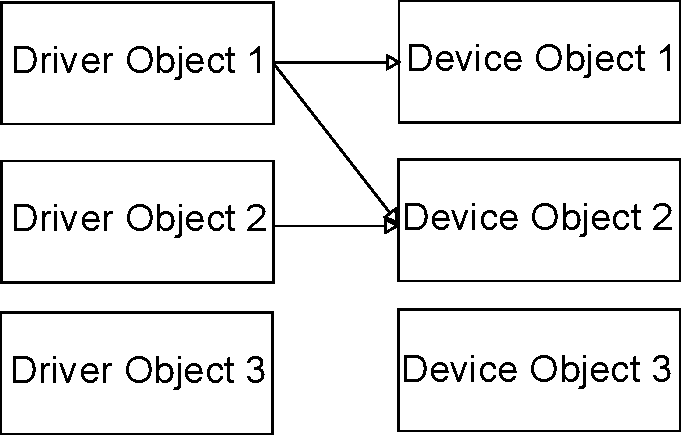
\includegraphics[width=0.6\linewidth]{./graph/drv-to-dev}
\caption{设备对象和驱动对象的对应关系}
\label{fig:drv-to-dev}
\end{figure}

WDM模型的驱动程序按功能可以分为三类:
\begin{enumerate}
\item
总线型:驱动某种类型的计算机总线,为这种总线上挂载的每个设备提供独立的功能接口。检测和处理总线上设备的挂载和移除事件。
\item
功能型:驱动某种特定类型的硬件设备,与设备进行交互,向应用程序提供硬件的访问接口。一般由硬件厂商提供,一个驱动程序可服务多个同类型的硬件设备。
\item
过滤器型:过滤针对某个、某种类型的设备或是总线的IO请求。过滤器驱动程序可以任意选择请求的处理方式:直接传递、处理后传递或是丢弃。
\end{enumerate}

实践证明,使用WDM模型开发硬件驱动程序会使系统内核更加稳定,操作系统可以更加有效地控制硬件。除了定义一个驱动程序与操作系统连接的标准接口以外,WDM还指明了驱动程序应该采用的更加模块化的体系架构。

\subsection{IRP和驱动程序堆栈}
IRP(I/O request package)是Windows内核中一种用于驱动程序模块之间交互的数据结构。上层应用程序通过调用一定的API函数与硬件设备交互,这使得IO管理器根据请求的类型产生相应的IRP。IRP被传递给驱动内部的分发函数进行处理,IO管理器最终将驱动程序返回的结果传递给应用程序。捕获IO操作的实质就是捕获IRP的操作。

驱动程序堆栈是从应用层到硬件的一整套设备驱动程序。大多数情况下,一个硬件设备能够正常运转依靠的是多个驱动程序的协同工作,这些驱动程序创建的设备对象按层次组合在一起,构成了设备的驱动程序堆栈。IRP通过每个设备所唯一对应的驱动程序堆栈传达至硬件本身。

\subsection{存储卷过滤器驱动}
任何设备的驱动程序堆栈都可以插入过滤器驱动程序。一个典型的驱动程序堆栈如图\ref{fig:io-stack-filter}所示,过滤器驱动程序不是设备运行所必须的,因此在图中以虚线画出。
\begin{figure}[H]
\centering
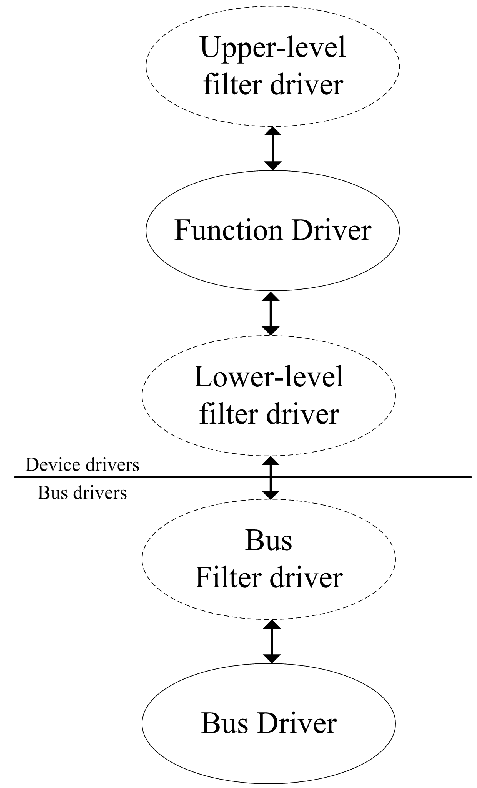
\includegraphics[width=0.4\linewidth]{./graph/io-stack-filter}
\caption{驱动程序堆栈和过滤器驱动程序}
\label{fig:io-stack-filter}
\end{figure}
除了功能型和总线型的驱动程序,存在三种类型的过滤器驱动程序。
\begin{enumerate}
\item
总线过滤器驱动:过滤、处理总线事件,将总线的硬件信号转换为驱动程序能够处理的总线事件,为总线设备加入新的功能。一种总线设备可存在多个总线过滤器驱动。
\item
底层过滤器驱动:位于功能型驱动程序之下,用于改变设备展现给功能型驱动程序的硬件行为。可存在多个底层过滤器驱动。
\item
上层过滤器驱动:位于功能型驱动程序之上,过滤应用程序发送给设备的IO请求。过滤到的IRP多为抽象程度高、硬件相关度低的IO请求。
\end{enumerate}

本论文实现的存储卷过滤器驱动程序,是一种存在于存储卷设备所属的驱动程序堆栈中的、上层过滤器型驱动程序。

\section{缓存页面替换算法}
\label{sec:cache_algorithm}

伴随着应程序访问存储设备,不断会有新的数据加入到缓存空间。当缓存中已经没有空闲的空间,而此时又有新的数据需要加入时,就需要使用缓存页面替换算法释放一定空间以容纳新的缓存数据。常用的缓存页面替换算法按照替换策略可分为三类,本缓存系统对这三种替换算法都进行了实现,运行时可选择其中任意一种:

\begin{enumerate}

\item 基于访问时间的LRU(Least Recently Used)系列替换算法

LRU替换算法依据缓存块最近一次的访问时间进行决策。当缓存没有空闲空间时,替换出最近最不使用的(距上次访问时间最长的)缓存块。

虽然LRU替换算法根据访问时间进行替换决策,但实现时并不需要为每个缓存块记录访问时间,而是使用链表的方式组织缓存块,使用缓存块在链表中的位置记录缓存块的访问先后顺序:链表存在冷、热两端,新缓存块由热端加入,运行中被访问的缓存块由链表中的某个位置移动到热端,需要时从链表的冷端移除缓存块。这样,从热端到冷端,链表中的元素按照最近一次访问时间递减的顺序排列。

LRU替换算法实现简单,能够很好的适应数据访问的变化。存在的缺点是没有考虑数据的长期访问特性。最近使用的缓存块可能并不会被经常访问,经常访问的数据可能因为暂时不使用而被换出,从而导致更需要留在缓存中的数据块被替换了出去。

\item 基于使用频度的LFU(Least Frequently Used)系列替换算法

LFU算法依据每个缓存块的访问频度进行决策。当缓存没有空闲空间时,替换出历史访问频率最低的缓存块。

新加入的缓存块初始访问频度为1,随系统运行动态调整访问频度。为了在最短时间找到被替换出的缓存块,实现中使用小顶堆数据结构进行缓存块的组织,堆顶元素总是访问频度最低的元素,随时可以被替换出去。

LFU算法需要为每个缓存块设置一个计数器,记录访问次数。使用了小顶堆数据结构实现替换策略,实现难度略高于LRU。缺点是需要一定策略对计数器进行清零,否则计数器只增不减会导致某些曾经被频繁访问的缓存块无法及时地被清理出去;新加入缓存块访问频度低,在缓存中停留较短时间就容易被替换出去。

\item 综合时间和频度的替换算法

在决定缓存中被替换的缓存块时,缓存替换算法只考虑最后一次的访问时间或使用频度某一项因素都会存在缺陷。为克服这种缺陷,本论文提出了一种综合考虑访问时间和使用频度的替换算法,该算法实现简单,且测试结果表明命中率优于LRU系列和LFU系列替换算法。以下是算法的处理逻辑:

\begin{itemize}
\item
替换算法使用冷、热两个链表管理缓存块(图\ref{fig:replace-algo-1}),初始状态下两个链表均为空。两个链表所能管理的空间之和代表了缓存的总容量。
\begin{figure}[H]
\centering
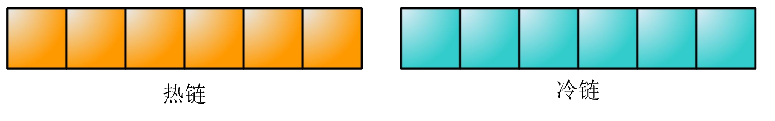
\includegraphics[width=0.6\linewidth]{./graph/replace-algo-1}
\caption{替换算法使用两个链表管理缓存块}
\label{fig:replace-algo-1}
\end{figure}

\item
当冷链表不为满时,新到来的缓存块首先会被加入到冷链表的热端,在运行过程中会统计每个缓存块访问的次数。图\ref{fig:replace-algo-2}展示了缓存块以A->B->C->D->E的字母表顺序加入后的缓存的组织状态状态。
\begin{figure}[H]
\centering
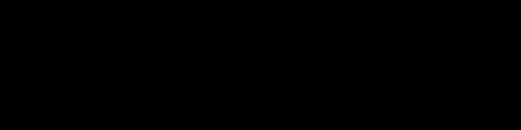
\includegraphics[width=0.6\linewidth]{./graph/replace-algo-2}
\caption{新到来的缓存块加入到冷链表}
\label{fig:replace-algo-2}
\end{figure}

\item
随着系统运行,缓存块会被不断加入。当冷链表已满,而又需要加入新的缓存块时。新的缓存块仍旧会被加入到冷链的热端,为腾出空间冷端就需要移出一个缓存块到临时空间。缓存算法会判断被移出缓存块的引用计数,如果其引用计数大于等于2,则清零其引用计数,并加入到热链表的热端;否则改缓存块占用的空间将会被释放。图\ref{fig:replace-algo-3}展示了加入块G移出块A的过程。
\begin{figure}[H]
\centering
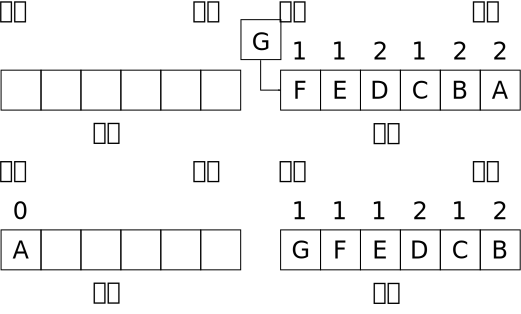
\includegraphics[width=0.6\linewidth]{./graph/replace-algo-3}
\caption{冷链表满时加入缓存块的处理策略}
\label{fig:replace-algo-3}
\end{figure}

\item
新缓存块的持续到来导致冷链表中的缓存块不断被移动到热链表,热链表也会逐渐变满。继续从冷链表向热链表移动缓存块会导致热链表的冷端的缓存块像图\ref{fig:replace-algo-3}中冷链表的冷端的缓存块一样被换出。这些被换出的缓存块的引用计数被清零后,被加入到冷链的热端,重复图\ref{fig:replace-algo-3}的过程。这一过程在图\ref{fig:replace-algo-4}中被描述。
\begin{figure}[H]
\centering
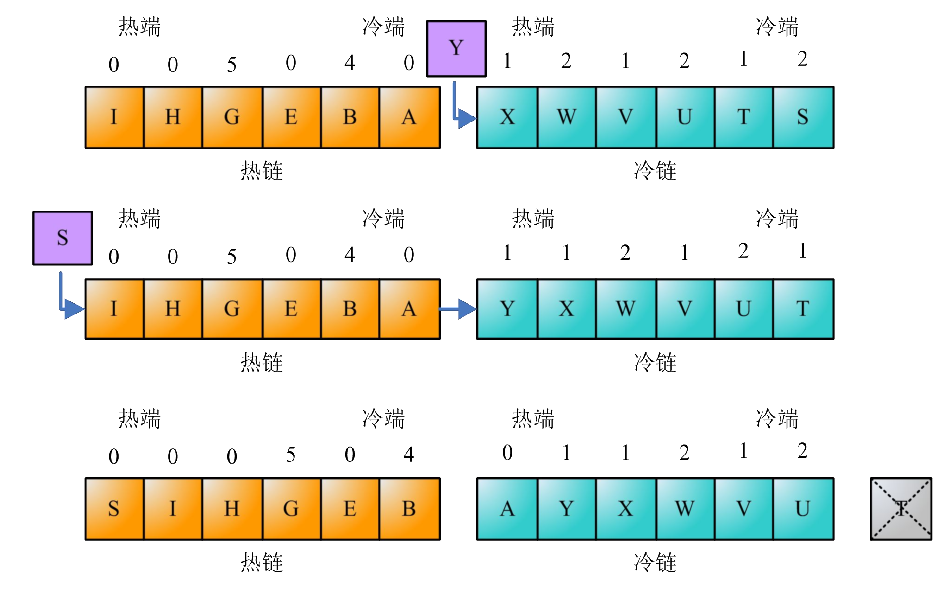
\includegraphics[width=0.7\linewidth]{./graph/replace-algo-4}
\caption{冷热链表均满时加入缓存块的处理策略}
\label{fig:replace-algo-4}
\end{figure}
\end{itemize}

\end{enumerate}

\section{缓存映射策略}
\label{sec:cache_mapping}

存在三种使用最为广泛的缓存映射策略。

\begin{enumerate}

\item 直接相联映射

主存储器中的每一块映射到缓存中的某个特定存储块中。缓存中的每个缓存块与主存中的一个或多个存储块相关联(图\ref{fig:cache-map-1})。

\begin{figure}[H]
\centering
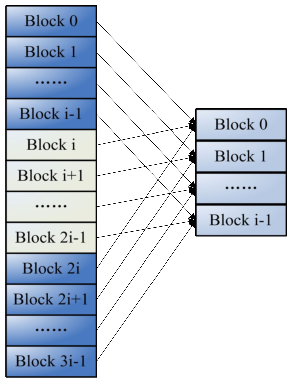
\includegraphics[width=0.3\linewidth]{./graph/cache-map-1}
\caption{直接相联映射}
\label{fig:cache-map-1}
\end{figure}

映射规则:
\begin{itemize}
\item 主存与缓存按照相同大小的数据块组织。
\item 主存容量应是缓存容量的整数倍。将主存空间按缓存的容量分成区,主存中每一区内的块数与缓存的总块数相等。 
\item 主存中某区的一块存入缓存时只能存入缓存中块号相同的位置。
\end{itemize}

设主存的第块i映射到缓存的第j块,则i和j满足如下关系。
j = i mod m	(m为主存每一区的总块数)
直接映射方式的优点是实现简单,可以使用主存地址直接计算出对应的缓存地址,不存在查找过程。缺点是缓存中的每个存储块通常对应主存中多个固定的存储块,运行中如果存在多个块同时被访问会产生缓存替换策略被频繁调用的情况。因此,直接映射适合缓存容量为主存的30\%以上时采用,一般应用于超大型系统。

\item 全相联映射

主存储器中的任意一块可以映射到缓存中的任意一块(图\ref{fig:cache-map-2})。

\begin{figure}[H]
\centering
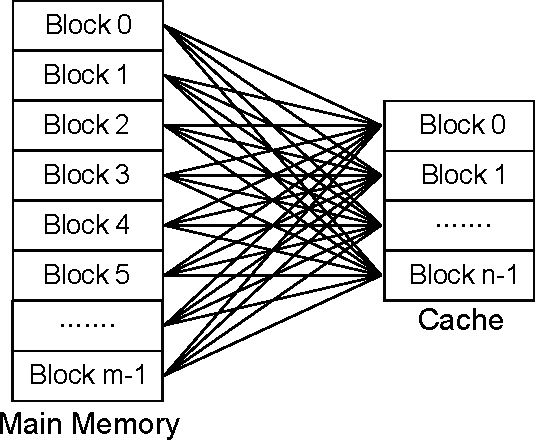
\includegraphics[width=0.3\linewidth]{./graph/cache-map-2}
\caption{全相联映射}
\label{fig:cache-map-2}
\end{figure}

映射规则:
\begin{itemize}
\item 主存与缓存按照相同大小的数据块组织。
\item 主存的某一数据块可以装入缓存的任意一块空间中。
当缓存块数为Cb,主存块数为Mb时,存在Cb×Mb种映射关系。
\end{itemize}

全相联映射的优点是主存和缓存的容量没有限制,只需按照相同大小的数据块进行组织。缺点是当查询主存中的某个数据块是否被缓存时,在不使用额外存储空间的情况下要遍历所有缓存块进行查找。为提高查找效率,可使用多种查找数据结构进行索引,但需要额外的存储空间。

\item 组相联映射

主储存器的每一组都与缓存中的某一组相对应,组内的每个块与缓存组内的任意一个存储块相映射(图\ref{fig:cache-map-3})。

映射规则:
\begin{itemize}
\item 主存与缓存按照相同大小的数据块组织。
\item 主存与缓存以同样的大小划分成组。
\item 主存容量是缓存容量的整数倍,将主存空间按缓存的容量分成区,主存中每一区内的块数与缓存的总块数相等。
\end{itemize}

\begin{figure}[H]
\centering
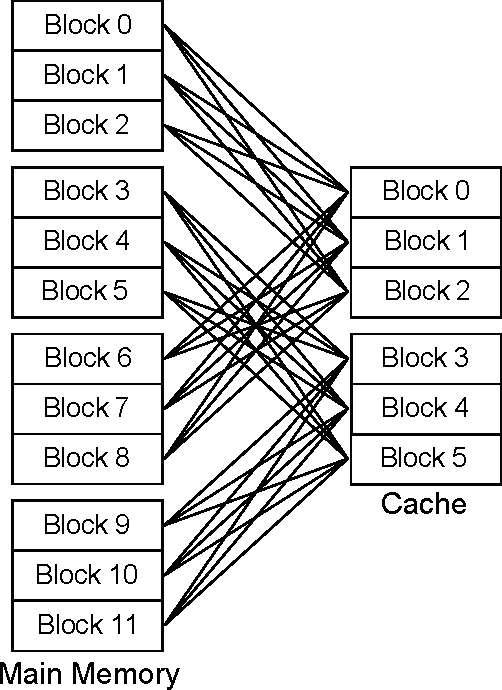
\includegraphics[width=0.4\linewidth]{./graph/cache-map-3}
\caption{组相联映射}
\label{fig:cache-map-3}
\end{figure}

当主存的数据转储到缓存中时,可以使用主存地址求出唯一对应的缓存组号,也就是主存组内的某一块只能存入同组号的缓存空间内。相关联的两组内各存储块之间则可以任意存放。从主存组到缓存组之间采用直接映射相联方式;在两个对应的组内采用全映射相联方式。

\end{enumerate}

一般从三个方面对不同的映射方式进行比较。
\begin{itemize}
\item 索引速度:直接映射可以直接计算出缓存地址,不需要查找,速度最快;组相联方式则需要查找对应的缓存组,速度次之;全映射的速度最慢。
\item
缓存利用率:全相联映射缓存块的映射是任意的,利用率最高;组相联方式组内映射任意,但是组间相互独立,利用率次之;直接映射缓存中的每个缓存块与主存中的一个或多个存储块相关联,利用率最低。
\item
实现难度:直接映射方式最简单,适合硬件实现;组相联方式和全映射方式的实现难度取决于使用的索引数据结构。当组内块数量较少时组相联方式可以使用遍历的方法,实现相对简单。
\end{itemize}

\section{缓存索引数据结构}
\label{sec:cache_indexing}

缓存系统使用的映射结构决定了缓存索引结构的选择。

使用直接映射结构,主存储器中的每个数据块,根据地址映射关系,对应了缓存中唯一的一个缓存块。因此,使用直接映射策略进行缓存块的查找,不需要额外的缓存索引结构,直接使用计算出的缓存块地址检查该主存块是否被缓存即可。

使用全相联映射结构,主存储器中的每个数据块和缓存中的每个数据块的存储地址之间没有任何的关系,这时就需要某种额外的索引数据结构定位主存储块映射的缓存块地址。

使用组相联映射结构,是直接映射和全相联映射结构两种方式的折中。组相联映射将主存储器和缓存空间分组的思想类似于直接映射,而相联两组内的主存块和缓存块之间的任意映射关系又等同于全相联映射的思想。缓存系统的设计者决定了分组的大小:当分组内缓存块数量较少时,可使用实现简单的遍历方法查找,不需要额外的索引数据结构;分组内缓存块数量较大时,则和全相联映射一样需要额外的索引数据结构。

\subsection{单级有序索引}
单级有序索引,顾名思义,就是只需要查询一级,便可以完成从主存储器地址到缓存地址空间的转换。通常使用数组和链表两种数据结构进行索引。

\begin{enumerate}
\item 数组方式

使用静态数组为缓存中的每一个缓存块建立一个索引标签,标签记录了缓存块映射所到的主存储块,未映射时标记为空。索引需要遍历数组元素进行查找。优点是实现简单。缺点是需要在初始化阶段给所有的缓存块建立索引标签,如果缓存空间大,则需要的空间太多,索引速度慢。
\item 链表方式

使用动态链表为每一个已经使用的缓存块建立一个索引标签,链表中的所有标签按照缓存地址的大小顺序排列。通过加入、删除和更新链表元素的方式实现缓存映射的更新。相对数组,链表使用的空间可以在运行时动态分配。但索引时仍需要遍历所有链表元素。
\end{enumerate}

\subsection{多级有序索引}

多级索引空间是对单级索引空间或者空间范围进行多级划分,解决超大数据量缓存空间的检索速度问题。多级索引由于其多级的结构特性,可以很好地利用计算机硬件资源的并行工作特性,如多核,磁盘阵列等,提高缓存块的检索效率。

多级索引的方法很多,不同种类的单级索引组合在一起就可以构成多种多级索引的方法。但每种索引方式的特性不同,如何将多种索引融合成一体构成一种高效的多级索引,是多级索引的一个研究方向。

\subsection{B+树索引}
B+树是一种树数据结构,通常用于数据库和操作系统的文件系统中。B+ 树的特点是其插入与修改拥有较稳定的对数时间复杂度。B+ 树元素自底向上插入,这与二叉树恰好相反。

\begin{itemize}

\item B+树的节点结构

B+树中,节点被表示为一组有序的元素和子指针。如果B+树的阶(order)是m,那么。除了根节点外的每个节点都包含最少m/2个最多m-1个元素。对于所有内部节点,子指针的数目总是比元素的数目多一个,内部节点的子指针指向其他节点。所有叶子都在相同的高度上,叶子节点的子指针的数目等同于元素的数目,叶子节点的子指针指向被索引的数据。图\ref{fig:bplus-tree}展示了一棵阶为4的B+树。

B+树内部节点的元素充当了其子树的分离值。例如,某个内部节点存在两分离值(元素)$a_1$和$a_2$,则其必须存在三个子指针指向其子树:左子树的所有节点的元素值均小于$a_1$,中间子树所有节点的元素值处于$[a_1,a_2)$区间,右子树的所有节点的元素值均大于等于$a_2$。

\item B+树的查找算法

B+树的查找算法和排序二叉树的查找方法类似:从根节点开始,自顶向下遍历树的节点,根据要查找数据的索引值决定选择分离值哪一边的子指针。使用子指针进入下一层的节点,重复查找,直到到达叶子节点。遍历叶子节点的所有元素,查找索引值,如果存在相同元素则找到,否则B+树中不存在查询索引。

\item B+树的插入算法

当节点内元素的树木不属于B+树节点结构的可接受的范围时,这个B+树节点处于违规状态。节点内元素的最小数目必须大于最大数目的一半。B+树的插入过程要处理节点违规的情况,插入过程为:
\begin{enumerate}
\item 根据索引值,查找要插入元素的叶子节点。
\item 将元素插入到叶子节点内的合适位置。
\item 如果此时的叶子节点没有处于违规状态,处理结束。
\item 如果此时的叶子节点存在过多的元素,则分裂成两个叶子节点,这两个节点拥有最小数目元素。分裂操作导致上一层节点的子指针数目增加一个,因此需要递归向上处理直到到达根节点。如果根节点也被分裂,则创建新的根节点,根节点的元素个数没有下限的要求。
\end{enumerate}

\item B+树的删除算法

B+树的删除过程要处理节点违规的情况,删除过程为:

\begin{enumerate}
\item 根据索引值,查找要删除元素的叶子节点。
\item 将叶子节点内的待删除元素删除。
\item 如果此时的叶子节点没有处于违规状态,处理结束。
\item 此时节点可能处于以下两种违规的状态之一,递归向上处理违规的叶子节点,直到不存在违规节点:
\begin{enumerate}
\item 节点的左、右兄弟节点,在不变为违规节点的前提下,可以把一或多个子节点移动到处于违规状态的节点,使其变为合法的节点。在移动子节点后更新父节点和兄弟节点的分离值,递归向上处理。
\item 节点的左、右兄弟节点内的元素个数均处于合法个数的下界。这种情况下,把左或右兄弟节点与处于违规状态的节点合并,再平均分裂为两个节点,更新父节点和兄弟节点的分离值,持续这一过程直到当前节点是合法状态或者到达根节点。
\end{enumerate}
\end{enumerate}

\end{itemize}

\begin{figure}[H]
\centering
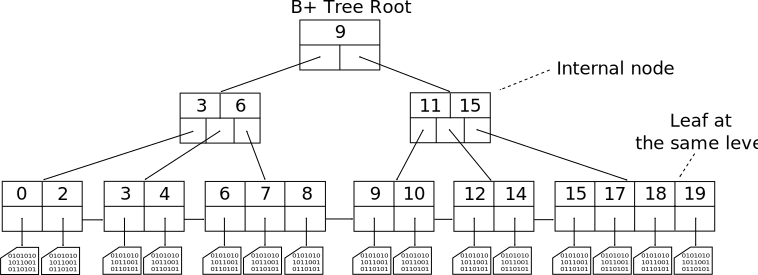
\includegraphics[width=1\linewidth]{./graph/bplus-tree}
\caption{B+树结构}
\label{fig:bplus-tree}
\end{figure}

\section{回写策略}
\label{sec:wb_strategy}

对于应用程序的读请求,HDD上的数据不会被改变,因此不存在数据一致性的问题。对于应用程序的写请求,需要决定是直接应用写操作到HDD还是延迟写。学术上存在三种回写策略:写穿法、写回法和写一次法。本系统实现了前两套处理方案。

\subsection{写穿法(Write Through)}
\begin{figure}[H]
\centering
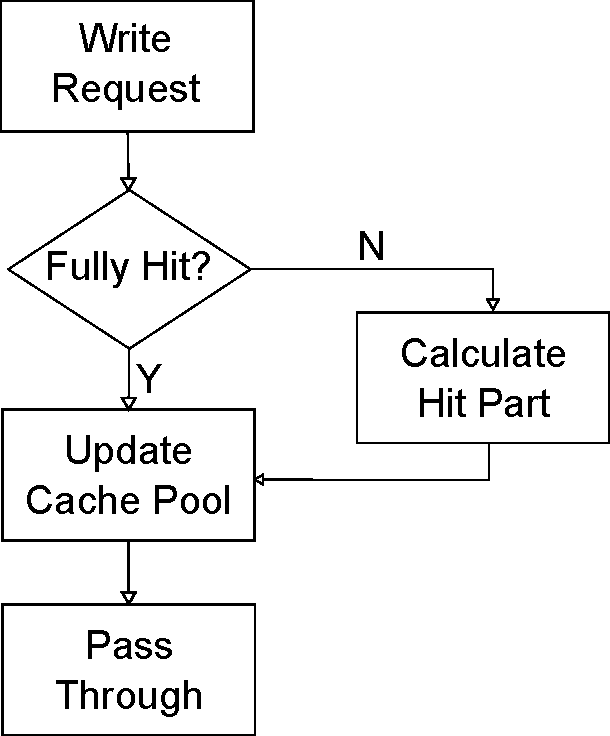
\includegraphics[width=0.4\linewidth]{./graph/write-through}
\caption{写穿法处理策略}
\label{fig:write-through}
\end{figure}

对于写请求,同时应用于HDD和SSD缓存。由于HDD和缓存是同时写入的,因此无需考虑数据一致性问题,也无需为每个缓存块设置标志位标记反映此块是否被修改过(图\ref{fig:write-through})。

\subsection{写回法(Write Back)}
\begin{figure}[H]
\centering
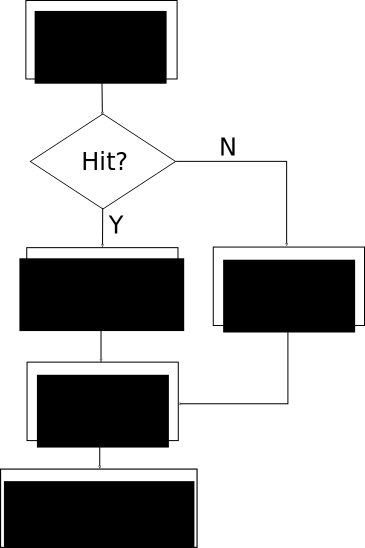
\includegraphics[width=0.4\linewidth]{./graph/write-back}
\caption{写回法处理策略}
\label{fig:write-back}
\end{figure}

对于写请求,在应用于SSD缓存后就结束请求。为每个缓存块设置修改标志,将标志为脏的缓存块加入回写队列(图\ref{fig:write-back-queue})。

\begin{figure}[H]
\centering
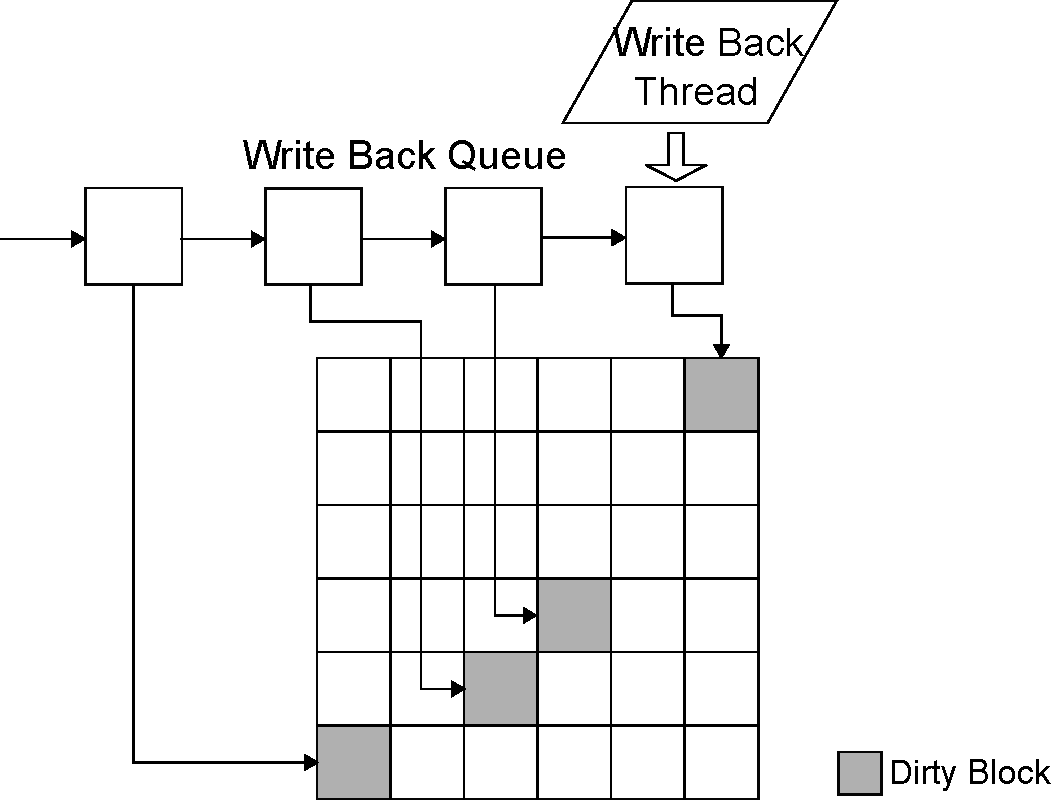
\includegraphics[width=0.4\linewidth]{./graph/write-back-queue}
\caption{指向脏数据块的回写队列}
\label{fig:write-back-queue}
\end{figure}

回写队列的大小是固定。随着脏数据块的加入,当回写队列满时,会触发回写线程进行回写操作。会写线程会将队列中的所有脏缓存块刷回HDD。同样的,当线程接收到回写所有或线程终止信号时,也会进行刷回所有脏缓存块到HDD的操作(图\ref{fig:write-back-thread})。

\begin{figure}[H]
\centering
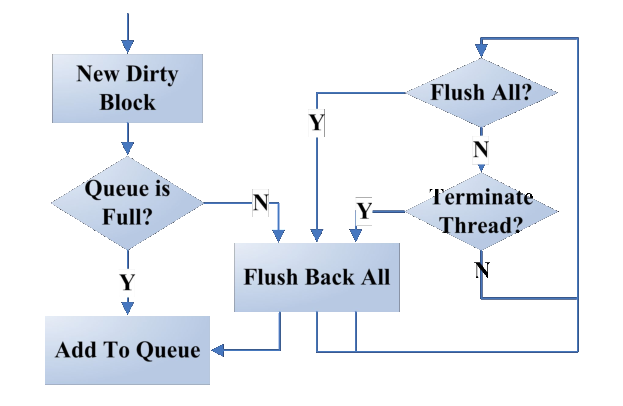
\includegraphics[width=0.6\linewidth]{./graph/write-back-thread}
\caption{回写线程的回写逻辑}
\label{fig:write-back-thread}
\end{figure}

%% ----------------------------------------------------------------------
%%% END OF FILE
%% ----------------------------------------------------------------------